\section{Vorwort}
Für den Support und Bereitstellung von Hardware bedanken wir uns herzlich bei Herrn Krinke von der pi4\_robotics GmbH Berlin und für die beratende Funktion danken wir den Dozenten und Professoren der Beuth Hochschule Prof. Löwis, Dr. Flemming und Prof. Görlich.\\
Bei der Recherche zur Bearbeitung des Projektes wurden viele englische Webseiten zu rate gezogen und auch die man-pages der meisten Programme sind in Englisch verfasst. Generell kann man sagen, dass englische Fachbegriffe sich im Bereich Software etabliert haben, so dass eine Übersetzung eher verwirren als helfen würde. Daher haben wir uns entschieden, die \textbf{englischen} Bezeichner und Beschreibungen von Flags und Optionen beizubehalten.\\
Um Codeabschnitte besser von Beschreibungen unterscheiden zu können, wurde eine eigene Schriftart verwendet:
\begin{verbatim}
  Kommandozeilen Eingaben und Codesnippets werden wie HIER dargestellt.
\end{verbatim}

\section{Projektbeschreibung}
Das erklärte Ziel der pi4\_robotics GmbH Berlin ist es humanoide Roboter weiter zu entwickeln. 
Diese können bereits in unterschiedlichen Branchen eingesetzt werden. Im Werbeblatt 
des Workerbot4 (siehe Anhang, Kapitel \ref{RefAnhang}) werden die Basisfähigkeiten des Jolandi Workerbot beschrieben.  \\
Bisher ist das Anlernen neuer Tätigkeiten und die Bedienung nur über eine PC-Schnittstelle möglich. Doch das soll sich ändern. Geplant ist Spracherkennung und visuelle Wahrnehmung 
zu integrieren, um mit dem Roboter wie mit einem Menschen kommunizieren zu können. Auch soll 
ein Avatar Modus implementiert werden, bei dem der User in die Rolle des Roboters schlüpft 
und per Teleoperation den Roboter bewegt, hört was der Roboter hört und mit den Augen des Roboters sieht. \\
\begin{minipage}{\textwidth}
    \begin{center}
        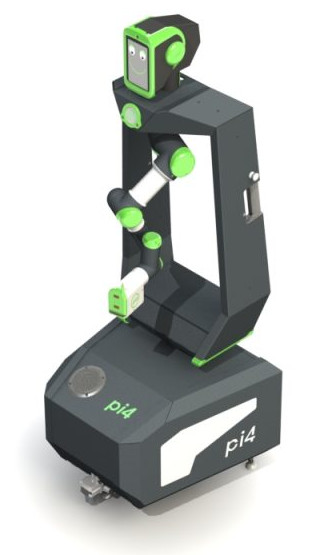
\includegraphics[scale=0.5]{img/jolandi.jpg} 
    \end{center}
\end{minipage}
\begin{center}
Jolandi Workerbot der Firma pi4\_robotics GmbH
\end{center}
 
\begin{minipage}{\textwidth}
    \begin{center}        
        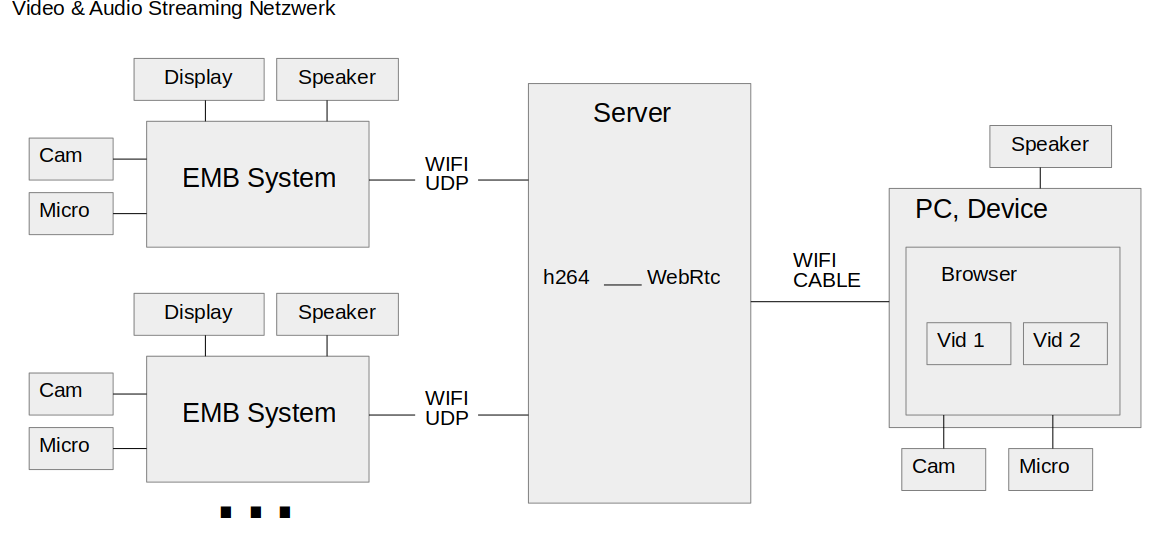
\includegraphics[scale=0.4]{img/schemaproj.png} 
    \end{center}
\end{minipage}
\begin{center}
Schemaplan der Komponenten
\end{center}
Für den Einsatz als Sicherheitspersonal ist weiterhin geplant, die Stimme des Bedieners aus dem Roboter Lautsprecher ertönen zu lassen und sein Gesicht auf dem Kopfdisplay anzuzeigen. 
Der Kunde soll das Gefühl haben, dass der Roboter der Avatar des Bedieners ist.\\
Für die Laborübungen 'Entwurf eingebetteter Systeme' und 'Netzwerk-Programmierung' wurde 
bidirektionale Ton und Video Übertragung ausgewählt. Dabei galt es Audio und Video \textbf{mehrerer} Roboter auf eine Webseite zu streamen und eine Webcam inklusive Ton des PC auf alle verbundenen Roboter zurück zu streamen.\\

Der Schemaplan zeigt den grundlegenden Aufbau des Komplettsystems. Auf der linken Seite sind 'n' integrierte eingebettete Systeme gezeigt, wie sie in pi4\_robotics GmbH Robotern verbaut sind. Pro Roboterkopf ist ein Raspberry PI mit Touch-Display vorhanden. Für das Projekt wurde jeweils eine Webcam für Ton und Video angeschlossen. Die Tonwiedergabe erfolgt über einen USB Lautsprecher. Die Anzeige des empfangenen Videostreams soll \textbf{ohne} Webbrowser erfolgen.\\
Auf der rechten Seite des Plans ist der Bediener PC dargestellt. Auch hier liefert eine Webcam Ton und Video. Der empfangene Audiostream wird über die PC Lautsprecher ausgegeben.\\
Für den Bediener soll ein \textbf{Web-Template} erstellt werden. Dort kann dieser auswählen, welcher Videostream angezeigt werden soll. Der Zeitversatz bei der Übertragung soll sehr gering sein 
(<0.2sek), damit der User möglichst schnell reagieren kann. Bildübertragung zum eingebetteten System darf einen leichten Zeitversatz haben, da dort nur das Gesicht des Bedieners angezeigt wird, aber keine weiteren Handlungen davon abhängen.\\
Das gesamte Streaming soll über das Internet erfolgen. Dabei ist der Datentransfer auch aus 
fremden WLAN Netzen heraus zu realisieren. Fremd im Sinne, dass die dazwischen liegenden Router und Ports nicht konfiguriert werden können. Die IP Adressen der Roboter sind damit quasi unbekannt, d.h. dynamisch wechselnd oder/und nicht vom Internet aus sichtbar, d.h. es ist nicht möglich direkt vom Sender zum Empfänger zu streamen.\\
Eine weitere Anforderung war, den Datentransport möglichst Effizient zu gestalten. Für den Upload ins Internet sollte ein Transportprotokoll mit geringem Overhead gewählt werden und für das Streaming auf die Webseite ein natives Format, welches von aktuellen Browsern unterstützt wird. Die Visualisierung sollte in Html5 \& Javascript ohne Browser-Plugins, Flash o.ä. erfolgen. Für die Realisierung musste also eine Möglichkeit gefunden werden, das Upload Format zu konvertieren und die Webseite mit einem Audio- und Videostream zu versorgen. Eine Streaminglösung über das Web erfordert drei Basiskomponenten um die Aufgabe zu erfüllen. Einen Streaming Server, einen Sender und einen Empfänger.

\textbf{Streaming-Server:} 
Ist die Hauptkomponente, die Audio- und Videoinhalte von den Sendern an die Empfänger weiterleitet. Gleichzeitig kann auch die Konvertierung von einem Format oder Codec in ein anderes erfolgen.

\textbf{Sender:} Eine Quelle, die einen Audio- und Videostream zum Server schickt. 

\textbf{Empfänger:} Ein Empfänger, der sich mit dem Stream vom Server verbindet und diesen abspielt oder speichert.